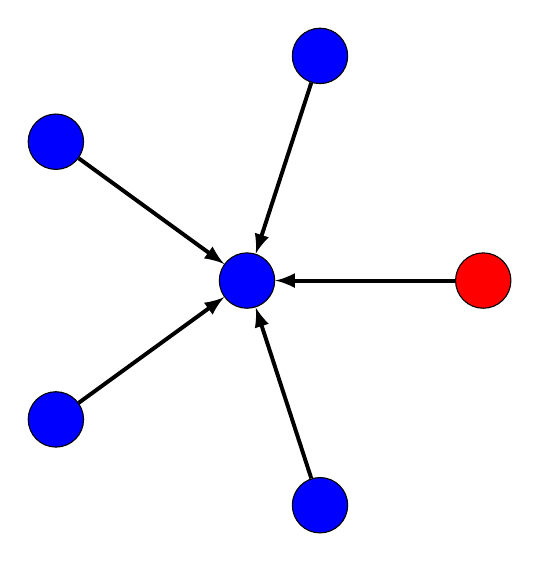
\begin{tikzpicture}
    \node[draw, fill=blue, circle, minimum size=20pt] (center) at (0, 0) {}; % Central node in blue
    
    \foreach \i in {1,...,5} {
        \ifnum\i=1
            \node[draw, fill=red, circle, minimum size=20pt] (n\i) at ({360/5 * (\i-1)}:3) {}; % First outer node in red
        \else
            \node[draw, fill=blue, circle, minimum size=20pt] (n\i) at ({360/5 * (\i-1)}:3) {}; % Other outer nodes in blue
        \fi
        \draw[->, line width=0.5mm, >=latex] (n\i) -- (center);
    }
\end{tikzpicture}